\chapter{Orbits}
In the following sections, we show that orbits are really conic sections. The case of a circular orbit is just a special case.
\section{Eliptical orbits}


\begin{figure}[h]
	\begin{center}
	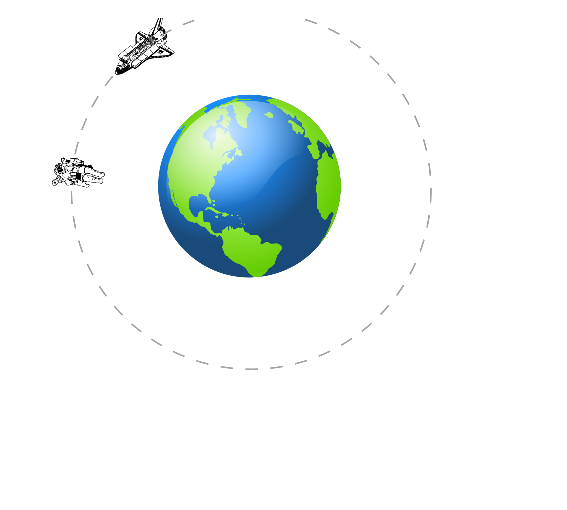
\includegraphics[width=0.5\textwidth]{orbit_figure}	
	\caption{A PH121 Circular Orbit, It's not Enough!}
\end{center}
\end{figure}


\begin{figure}[h]
	\begin{center}
		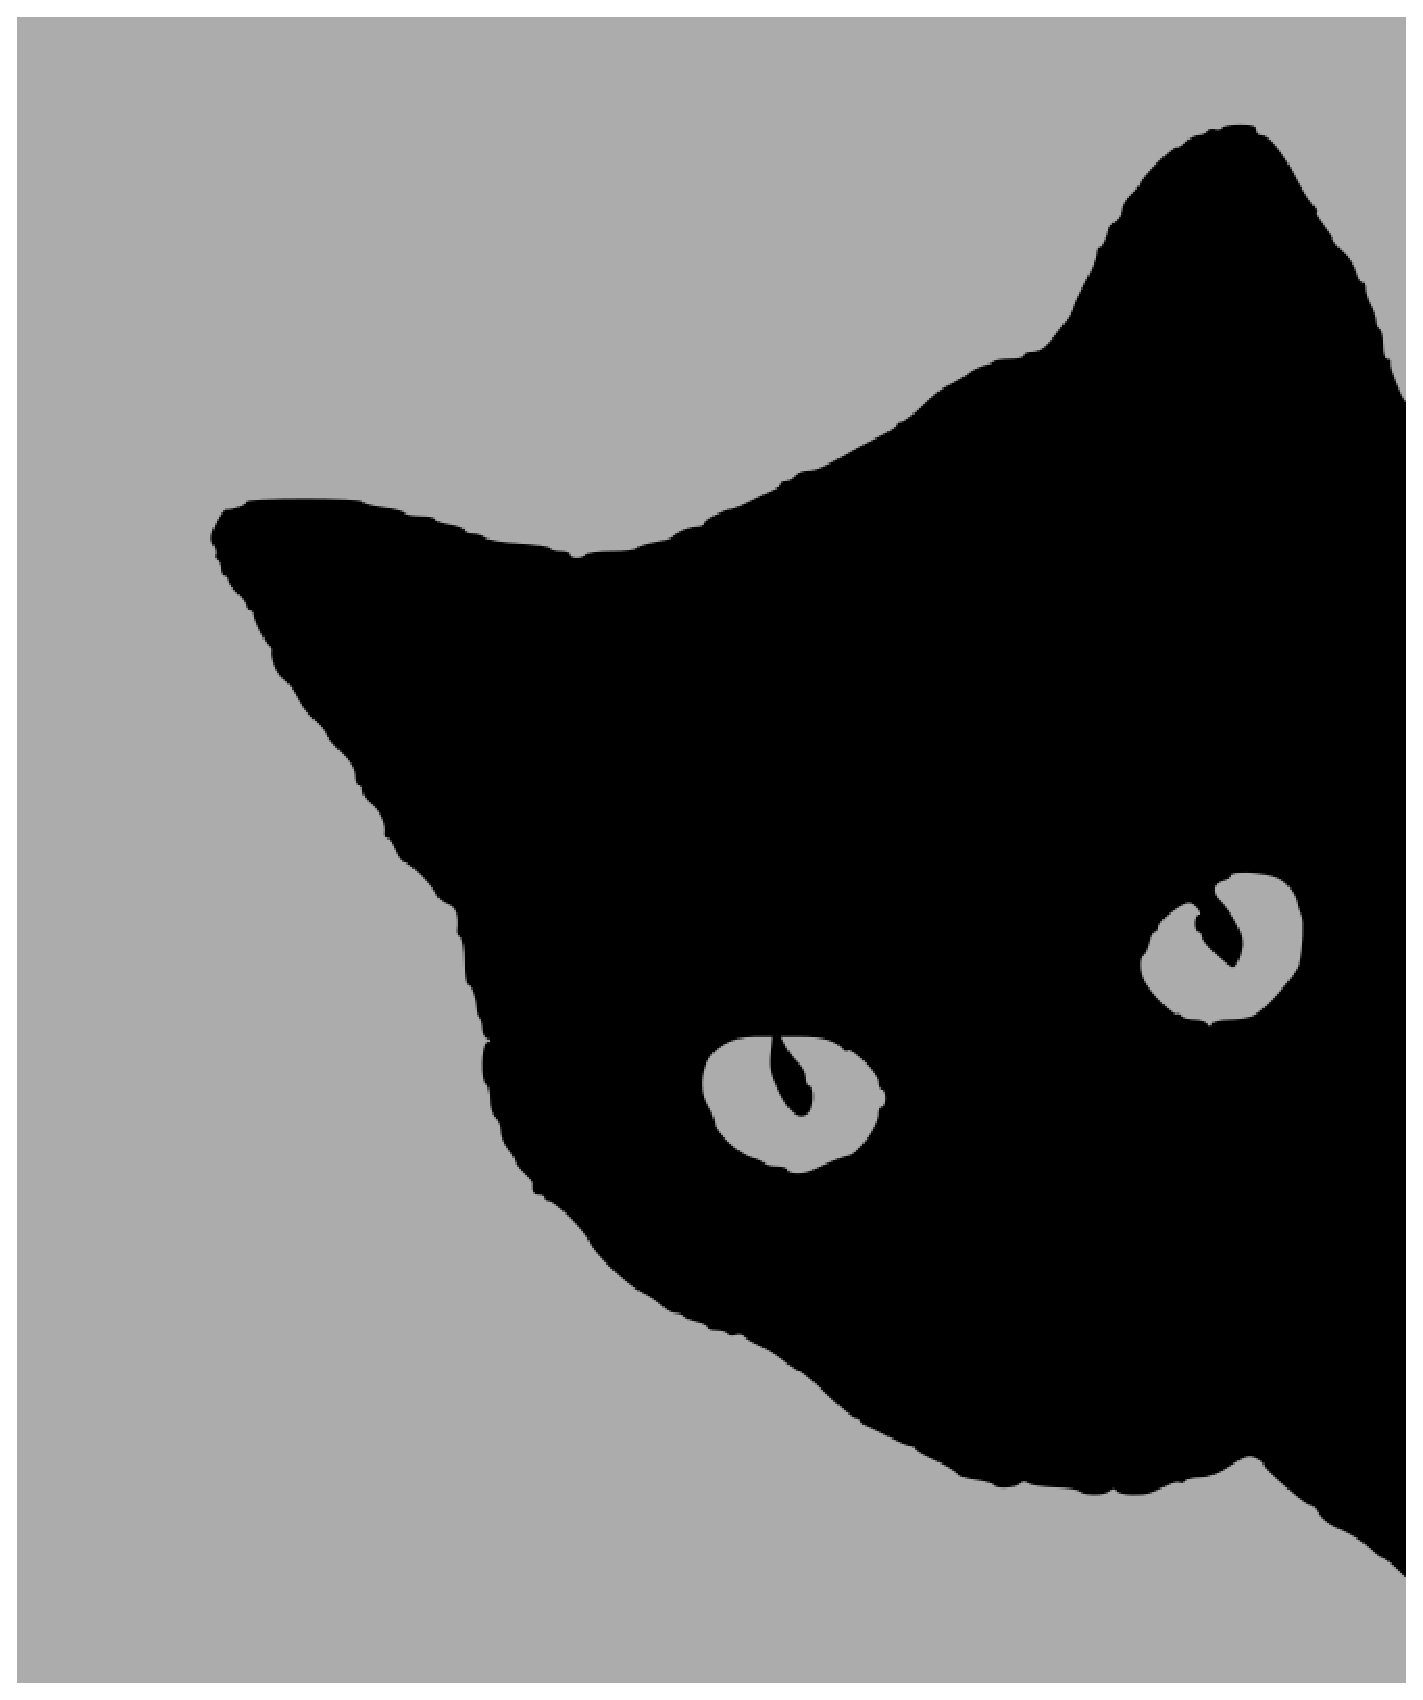
\includegraphics[width=0.5\textwidth]{cat}	
		\caption{A mistake}
	\end{center}
\end{figure}

In all our work in PH121 we used circular orbits. Kepler said orbits

should be elliptical. And that is true. We won't go though this in class,

but showing that Newton's law of gravitation implies an ellipse is a great

way to show off our new mathematics of dot and cross products. So if you are

comfortable with our new math, and curious to see how orbits work, read on.


Let's start with Newton's second law for our orbiting satellite again.

\begin{align*}
\overrightarrow{W}&=-m_{s}\overrightarrow{a}\\
&=-m_{s}g\left( r\right) \hat{r}\\
&=-m_{s}\left( G\frac{M_{E}}{r_{Es}^{2}}\right) \hat{r}
\end{align*}




We can write this as 

$$
-m_{s}\overrightarrow{a}-m_{s}\left( G\frac{M_{E}}{r_{Es}^{2}}\right) \hat{r}=0
$$


The subscripts may become burdensome, so we will drop them now, but remember

that $r=r_{Es}$ is the distance from the satellite to the Earth center of

mass to center of mass. 

$$-m_{s}\overrightarrow{a}-m_{s}\left( G\frac{M_{E}}{r^{2}}\right) \hat{r}=0$$

In the next section we will find that conservation of energy is important \ref{ConservationEnergy}. Notice that I used a marker to come up with the section number automatically.

\section{Conservation of Orbital Mechanical Energy\label{ConservationEnergy}}


Now we are going to do something strange. For no apparent reason, lets

compute the dot product of both sides of this equation 

$$\overrightarrow{v}\cdot \left( m_{s}\overrightarrow{a}+m_{s}\left( G\frac{M_{E}}{r^{2}}\right) \hat{r}\right) =\overrightarrow{v}\cdot 0 $$

then 

$$\overrightarrow{v}\cdot m_{s}\overrightarrow{a}+\overrightarrow{v}\cdot m_{s}\left( G\frac{M_{E}}{r^{2}}\right) \hat{r}=0 $$

or

$$m_{s}\overrightarrow{v}\cdot \overrightarrow{a}+m_{s}\left( G\frac{M_{E}}{r^{2}}\right) \overrightarrow{v}\cdot \hat{r}=0 $$

Now we need to learn a little bit more about dot products mixed with

derivatives. We have a position vector $\overrightarrow{r}=r\hat{r}$ The

derivative of this position vector is 

$$\frac{d\overrightarrow{r}}{dt}=\frac{d}{dt}\left( r\hat{r}\right) $$

$$=r\frac{d\hat{r}}{dt}+\frac{dr}{dt}\hat{r}$$


so if we take 

$$\frac{d\overrightarrow{r}}{dt}\cdot \hat{r}=\left( r\frac{d\hat{r}}{dt}+\frac{dr}{dt}\hat{r}\right) \cdot \hat{r}$$


$$=r\frac{d\hat{r}}{dt}\cdot \hat{r}+\frac{dr}{dt}\hat{r}\cdot \hat{r}$$%

$$=0+\frac{dr}{dt}$$%

since $d\hat{r}/dt=0.$


So 

$$\frac{d\overrightarrow{r}}{dt}\cdot \hat{r}=\frac{dr}{dt}$$

and we recognize 

\begin{equation*}
	\overrightarrow{v}=\frac{d\overrightarrow{r}}{dt}
\end{equation*}%
so we can write 
\begin{equation}
	\overrightarrow{v}\cdot \hat{r}=\frac{dr}{dt}  \label{vdotrhat}
\end{equation}%
and we have this in our orbit equation. Our orbit equation becomes

\begin{equation*}
	m_{s}\overrightarrow{v}\cdot \overrightarrow{a}+m_{s}\left( G\frac{M_{E}}{%
		r_{Es}^{2}}\right) \frac{d\overrightarrow{r}}{dt}\cdot \hat{r}=0
\end{equation*}%
or just

\begin{equation*}
	m_{s}\overrightarrow{v}\cdot \overrightarrow{a}+m_{s}\left( G\frac{M_{E}}{%
		r^{2}}\right) \frac{dr}{dt}=0
\end{equation*}

We can do something similar for the first term We can recognize 

$$\overrightarrow{a}=\frac{d\overrightarrow{v}}{dt}$$

and that $\overrightarrow{v}=v\hat{v}$ where $\hat{v}$ is a unit vector in

the same direction $\overrightarrow{v}.$ Then 

$$\frac{d\overrightarrow{v}}{dt}=\frac{d}{dt}\left( v\hat{v}\right) $$

$$=v\frac{d\hat{v}}{dt}+\frac{dv}{dt}\hat{v}$$

and 

$$\overrightarrow{v}\cdot \overrightarrow{a}=\overrightarrow{v}\cdot \frac{d\overrightarrow{v}}{dt}$$

$$=\overrightarrow{v}\cdot \left( v\frac{d\hat{v}}{dt}+\frac{dv}{dt}\hat{v}\right)
$$

$$=v\hat{v}\cdot v\frac{d\hat{v}}{dt}+v\hat{v}\cdot \frac{dv}{dt}\hat{v}$$

$$=0+v\frac{dv}{dt}\hat{v}\cdot \hat{v}$$

$$=v\frac{dv}{dt}$$

so our orbit equation becomes

$$m_{s}v\frac{dv}{dt}+m_{s}\left( G\frac{M_{E}}{r_{Es}^{2}}\right) \frac{dr}{dt}=0
$$
Now let's play a clever mathematical trick. Let's take the derivative of the
kinetic energy with respect to time.

$$\frac{d}{dt}\left( \frac{1}{2}mv^{2}\right) =\frac{1}{2}m\frac{d}{dt}\left(v^{2}\right) 
$$%
$$=\frac{1}{2}m\left( 2v\frac{dv}{dt}\right) 
$$%
$$=mv\frac{dv}{dt}$$%
Notice that this is in our orbit equation! So then%

$$m_{s}v\frac{dv}{dt}+m_{s}\left( G\frac{M_{E}}{r^{2}}\right) \frac{dr}{dt}=0
$$%
becomes 

$$\frac{d}{dt}\left( \frac{1}{2}mv^{2}\right) +m_{s}\left( G\frac{M_{E}}{r^{2}}\right) \frac{dr}{dt}=0$$%
We can play this trick again for the second term%

$$
\frac{d}{dt}\left( G\frac{M_{E}}{r}\right) =GM_{E}\frac{d}{dt}\left( \frac{1}{r}\right) 
$$
	
$$
=GM_{E}\left( -\frac{1}{r^{2}}\frac{dr}{dt}\right) 
$$
which once again we recognize this as part of our orbit equation so we can

write 

$$\frac{d}{dt}\left( \frac{1}{2}mv^{2}\right) -m_{s}\frac{d}{dt}\left( G\frac{M_{E}}{r}\right) =0$$

or 

$$\frac{d}{dt}\left( \left( \frac{1}{2}mv^{2}\right) -m_{s}\left( G\frac{M_{E}}{r}\right) \right) =0 
$$%
which tells us that 

$$
\left( \frac{1}{2}mv^{2}\right) -m_{s}\left( G\frac{M_{E}}{r_{Es}}\right) =\text{constant} 
$$
That is, the mechanical energy is conserved since we recognize this as just 
$$K+U_{g}=\text{constant} $$

And this makes sense. There are no energy loss mechanisms in our orbit. Our

masses are particles (no tidal forces inside the objects, etc.) So we expect

conservation of energy in forming our orbit.


\section{Conservation of Orbital Angular Momentum}


Now, let's do just what we did before only let's use a cross product with 
$\overrightarrow{r}$. 

$$\overrightarrow{r}\times \left( -m_{s}\overrightarrow{a}-m_{s}\left( G\frac{M_{E}}{r^{2}}\right) \hat{r}\right) =\overrightarrow{r}\times 0
$$

$$-\overrightarrow{r}\times m_{s}\overrightarrow{a}-\overrightarrow{r}\times m_{s}\left( G\frac{M_{E}}{r^{2}}\right) \hat{r}=0
$$

$$m_{s}\overrightarrow{r}\times \overrightarrow{a}+m_{s}G\frac{M_{E}}{r^{2}}\overrightarrow{r}\times \hat{r}=0
$$

$$m_{s}\overrightarrow{r}\times \overrightarrow{a}+m_{s}G\frac{M_{E}}{r^{2}}r\hat{r}\times \hat{r}=0
$$

The last term has $\hat{r}\times \hat{r}.$ The angle between $\hat{r}$ and $\hat{r}$ must be zero (they are in the same direction) so 
$$\hat{r}\times \hat{r}=\left( 1\right) \left( 1\right) \sin \left( 0\right) =0$$

and we are left with 

$$m_{s}\overrightarrow{r}\times \overrightarrow{a}=0$$

which really does note seem to helpful, but it is. Consider that 

$$\overrightarrow{a}=\frac{d^{2}\overrightarrow{r}}{dt^{2}}$$

so 

$$\overrightarrow{r}\times \overrightarrow{a}=\overrightarrow{r}\times \frac{d^{2}\overrightarrow{r}}{dt^{2}}$$

$$=\overrightarrow{r}\times \frac{d^{2}\left( r\hat{r}\right) }{dt^{2}}$$


Now consider the quantity 

$$\frac{d}{dt}\left( \overrightarrow{r}\times \frac{d\overrightarrow{r}}{dt}\right)=\overrightarrow{r}\times\frac{d^{2}\overrightarrow{r}}{dt^{2}}+\frac{d\overrightarrow{r}}{dt}\times \frac{d\overrightarrow{r}}{dt}$$

The second term must be zero because the angle between any vector and itself

must be zero and $\sin \left( 0\right) =0$, but the first term is just what

we have in our equation! so our equation becomes%

$$m_{s}\overrightarrow{r}\times \overrightarrow{a}=m_{s}\frac{d}{dt}\left( \overrightarrow{r}\times \frac{d\overrightarrow{r}}{dt}\right) =0$$

which we can write as%

$$\frac{d}{dt}\left( \overrightarrow{r}\times m_{s}\frac{d\overrightarrow{r}}{dt}\right) =0$$

$$\frac{d}{dt}\left( \overrightarrow{r}\times m_{s}\overrightarrow{v}\right) $$



$$=\frac{d}{dt}\left( \overrightarrow{L}\right) =0$$

and, hurray! we have conservation of angular momentum for our general orbit!


\section{Conic Section Equation}
You may not be a thrilled as I\ was at this point, but what we have done is typical for physicists. We use the power of mathematics and some ingenuity to predict what motions will be. You might say, \textquotedblleft but I\  would never think of taking cross and dot products seemingly randomly to find a result.\textquotedblright\ This may be true now, but as you get used to using the mathematical tools an operation like this may become more obvious. In any case, recall that early physicists spent many years trying out ways to use their mathematical tools. So eventually someone was bound to try our cross and dot product tricks. But we have only shown conservation of energy and angular momentum. We have not reached our goal. So let's return to our basic motion equation that we started with 
\begin{equation*}
	-m_{s}\overrightarrow{a}-m_{s}\left( G\frac{M_{E}}{r^{2}}\right) \hat{r}=0 
\end{equation*}
and now let's consider our equation for angular momentum
\begin{equation*}
	\overrightarrow{L}=\overrightarrow{r}\times m_{s}\overrightarrow{v}
\end{equation*}
and form the cross product of the first equation with $\overrightarrow{L}$
\begin{equation*}
	\left( -m_{s}\overrightarrow{a}-m_{s}\left( G\frac{M_{E}}{r^{2}}\right) \hat{%
		r}\right) \times \overrightarrow{L}=0\times \overrightarrow{L}
\end{equation*}
\begin{equation*}
	m_{s}\overrightarrow{a}\times \overrightarrow{L}+m_{s}\left( G\frac{M_{E}}{%
		r^{2}}\right) \hat{r}\times \overrightarrow{L}=0 
\end{equation*}
Again this may not seem like an obvious thing to do! But we find that
\begin{equation*}
	m_{s}\overrightarrow{a}\times \overrightarrow{L}=-\left( G\frac{M_{E}}{r^{2}}%
	\right) \hat{r}\times \overrightarrow{L}
\end{equation*}
and it is time for another mathematical trick. Consider the quantity
\begin{equation*}
	\frac{d}{dt}\left( \overrightarrow{v}\times \overrightarrow{L}\right) =%
	\overrightarrow{v}\times \frac{d\overrightarrow{L}}{dt}+\frac{d%
		\overrightarrow{v}}{dt}\times \overrightarrow{L}
\end{equation*}
\begin{equation*}
	=\overrightarrow{v}\times \frac{d}{dt}\left( \overrightarrow{r}\times m_{s}%
	\overrightarrow{v}\right) +\overrightarrow{a}\times \overrightarrow{L}
\end{equation*}
\begin{equation*}
	=\overrightarrow{v}\times \left( 0\right) +\overrightarrow{a}\times 
	\overrightarrow{L}
\end{equation*}
\begin{equation*}
	=\overrightarrow{a}\times \overrightarrow{L}
\end{equation*}
for our situation because we have already shown that angular momentum is
conserved. So we have
\begin{equation*}
	m_{s}\frac{d}{dt}\left( \overrightarrow{v}\times \overrightarrow{L}%
	\right)=-\left( G\frac{M_{E}}{r^{2}}\right) \hat{r}\times \overrightarrow{L}
\end{equation*}
Now let's look at the right hand side. Writing out the angular momentum gives
\begin{equation*}
	\hat{r}\times \overrightarrow{L}=\hat{r}\times \left( \overrightarrow{r}%
	\times m_{s}\overrightarrow{v}\right) 
\end{equation*}
and I will use a vector product identity that I\ will let the math department teach you
\begin{equation*}
	\overrightarrow{A}\times \left( \overrightarrow{B}\times \overrightarrow{C}%
	\right) =\overrightarrow{B}\left( \overrightarrow{A}\cdot \overrightarrow{C}%
	\right) -\overrightarrow{C}\left( \overrightarrow{A}\cdot \overrightarrow{B}%
	\right) 
\end{equation*}%
so for us
\begin{equation*}
	\overrightarrow{r}\times \overrightarrow{L}=m_{s}\hat{r}\times \left( 
	\overrightarrow{r}\times \overrightarrow{v}\right) 
\end{equation*}%
\begin{equation*}
	=m_{s}\left( \overrightarrow{r}\left( \hat{r}\cdot \overrightarrow{v}\right)
	-\overrightarrow{v}\left( \hat{r}\cdot \overrightarrow{r}\right) \right) 
\end{equation*}%
\begin{equation*}
	=m_{s}\left( \overrightarrow{r}\left( \hat{r}\cdot \overrightarrow{v}\right)
	-\overrightarrow{v}r\right) 
\end{equation*}%
We already know from equation (\ref{vdotrhat}) that%
\begin{equation*}
	\overrightarrow{v}\cdot \hat{r}=\frac{dr}{dt}
\end{equation*}%
then 
$$\hat{r}\times \overrightarrow{L}=m_{s}\left( r\hat{r}\left( \frac{dr}{dt}\right) -\overrightarrow{v}r\right) $$
then finally 
$$ m_{s}\frac{d}{dt}\left( \overrightarrow{v}\times \overrightarrow{L}\right)=-\left( G\frac{M_{E}m_{s}}{r^{2}}\right) \left( r\hat{r}\left( \frac{dr}{dt}\right) -\overrightarrow{v}r\right) 
$$
$$=-\left( GM_{E}m_{s}\right) \left[ \left( \frac{dr}{dt}\right) \frac{\hat{r}}{r}-\frac{\overrightarrow{v}}{r}\right] $$
Let's employ one more mathematical trick
$$\frac{d}{dt}\left( \frac{\overrightarrow{r}}{r}\right) =-\overrightarrow{r} \frac{1}{r^{2}}\frac{dr}{dt}+\frac{1}{r}\frac{d\overrightarrow{r}}{dt}
$$
$$=-\overrightarrow{r}\frac{1}{r^{2}}\frac{dr}{dt}+\frac{1}{r}\overrightarrow{v}
$$
$$=-\left( \hat{r}\frac{1}{r}\frac{dr}{dt}-\frac{1}{r}\overrightarrow{v}\right)$$
and this is the part of our equation that I\ wrote in square brackets, so with a substitution our equation becomes
$$m_{s}\frac{d}{dt}\left( \overrightarrow{v}\times \overrightarrow{L}\right)=\left( GM_{E}m_{s}\right) \left( \frac{d}{dt}\left( \frac{\overrightarrow{r}}{r}\right) \right) $$
or, canceling the $dt$ factors from both sides
$$m_{s}d\left( \overrightarrow{v}\times \overrightarrow{L}\right) =\left(GM_{E}m_{s}\right) \left( d\left( \frac{\overrightarrow{r}}{r}\right)\right)
$$
and we can integrate both sides
$$m_{s}\int d\left( \overrightarrow{v}\times \overrightarrow{L}\right)=-\left( GM_{E}m_{s}\right) \int \left( d\left( \frac{\overrightarrow{r}}{r}\right) \right)
$$
to find 
$$m_{s}\overrightarrow{v}\times \overrightarrow{L}=\left( GM_{E}m_{s}\right)\left( \frac{\overrightarrow{r}}{r}\right) +\overrightarrow{B}
$$
where $\overrightarrow{B}$ is a vector constant of integration. Once again for no apparent reason let's take the dot product of this equation with $\overrightarrow{r}$
$$\overrightarrow{r}\cdot \left( m_{s}\overrightarrow{v}\times \overrightarrow{L}\right) =-\left( GM_{E}m_{s}\right) \overrightarrow{r}\cdot \left( \frac{\overrightarrow{r}}{r}\right) +\overrightarrow{r}\cdot \overrightarrow{B} 
$$
and use another vector product identity
$$\overrightarrow{A}\cdot \overrightarrow{B}\times \overrightarrow{C}=\overrightarrow{A}\times \overrightarrow{B}\cdot \overrightarrow{C} 
$$
We can write this as to write our dot product equation as 
$$\left( m_{s}\overrightarrow{r}\times \overrightarrow{v}\right) \cdot \overrightarrow{L}=\left( GM_{E}m_{s}\right) r+rB\cos \theta _{rB} 
$$
or
$$\frac{1}{m_{s}}\left( \overrightarrow{r}\times m_{s}\overrightarrow{v}\right) \cdot \overrightarrow{L}=\left( GM_{E}m_{s}\right) r+rB\cos \theta_{rB}
$$
$$\left( \overrightarrow{r}\times m_{s}\overrightarrow{v}\right) \cdot \overrightarrow{L}=\left( GM_{E}m_{s}\right) r+rB\cos \theta _{rB} 
$$
$$\overrightarrow{L}\cdot \overrightarrow{L}=\left( GM_{E}m_{s}\right)r+rB\cos \theta _{rB} 
$$
$$L^{2}=\left( GM_{E}m_{s}\right) r+rB\cos \theta _{rB} 
$$
and now we can solve for $r$
$$L^{2}=r\left( \left( GM_{E}m_{s}\right) +B\cos \theta _{rB}\right) 
$$
then 

$$r=\frac{L^{2}}{\left( \left( GM_{E}m_{s}\right) +B\cos \theta _{rB}\right) } 
$$
or, rearranging slightly, 
$$r=\frac{L^{2}/\left( GM_{E}m_{s}\right) }{\left( 1+\left(B/GM_{E}m_{s}\right) \cos \theta _{rB}\right) } $$
If we compare this to the parametric equation for a conic section (straight out of your calculus text book), 
$$r=\frac{p}{1+e\cos \nu } $$
we can see that our orbit must be a conic section with a semi-latus rectum, 
$$p=L^{2}/\left( GM_{E}m_{s}\right) $$
and an eccentricity, 
$$e=B/GM_{E}m_{s}$$
and an angle 
$$\nu =\theta _{rB}$$
This means our orbit could be any conic section, circle, ellipse, parabola, or hyperbola. For satellites we most often choose ellipses. But the other conic sections are possible.So Kepler was partially right. An ellipse is a general form for an orbit, but it might even be better to write Kepler's law to say that orbits are conic sections.

If you are a normal PH121 student, your reaction to this problem might be \textquotedblleft Agh, maybe I should change my major to horticulture!\textquotedblright\ But don't worry, This was really a junior level problem, and for us physics majors we have many classes (both physics and math classes) to take before we would be expected to do a problem like this. Still it is fun to see that we \emph{can} do a problem like this with the math we learned in lowly PH121 if we are very persistent!  Interested students can read more in the the book \textit{Fundamentals of Astrodynamics} by Bate \textit{et. al.} \cite{Bate1971}\cite{ExplainingComputers2021}\cite{byuiphysics}\cite{Acquista76}
	
